\chapter{Focus sur des sous-parties du modèle}

\section{Structures des activités agropastorales}

\begin{paracol}{2}
Les participants ont fait le choix de distinguer les rôles de pasteur et d'agriculteur tout en soulignant qu'ils pouvaient tout à fait être endossés par la même personne. Nous y reviendrons plus loin, mais il est intéressant de constater qu'une grande part des conflits sont le fait des divergences d'intérêt de ces deux rôles. La superposition des deux rôles en un même acteur (agro-pasteur) concourt à une plus grande stabilité du système et au partage d'une certaine empathie, les enjeux des deux rôles étant accessibles à la même personne.

\switchcolumn %Sérères

We I mbaxtaan ta ndeta ba a ngadji ke o kaynaak oxe fo o koxoox oxe a warna o fia, bo da lay e, nam cialel pogrer oo nda o kin oleng a waa djialan, yam a diega solo I and ee a niox ake na diegaa nder den dik kaa sob ee entere ke den kaa mbog ree, nda o sobangayee o kiin o leng oxe na fia dik ke ndawir dieg kee

\switchcolumn %Francais

Dans la figure \ref{fig:agripasteur}, nous nous sommes intéressés aux réseaux égocentrés de l'agriculteur et de l'éleveur. Nous nous intéressons donc aux connexions directes que ces deux rôles entretiennent.

Les agriculteurs, comme les éleveurs, font partie des cuisines qui sont elles-mêmes sous l'autorité du chef de cuisine et du chef de concession. Ces deux rôles participent et contribuent à assurer la paix sociale.

\switchcolumn %Sérères

No natal \ref{fig:agripasteur} ke soxal na in ten refu ee lokoor ne djiegna nder o koxoox oxe fo o kaynaak oxe.

Den dik fop no ngaak a ngeenu to a niowaa no niuxur no waal ngaak ne ne mbaat no waal mbind ne ne, to wiin dik wene kaa mbexey aa diam a djieg.

\switchcolumn %Francais

Cette paix sociale en temps qu'élément liant du système est importante à caractériser, tant pour l'analyse du système que du point de vue des acteurs qui le constituent : les participants ont volontiers considéré la paix sociale comme un outil de production. Cette paix sociale est également territorialisée, et l'intensité des comportements qui s'y rapportent varie en conformité avec la première loi de la géographie de Tobler : “tout interagit avec tout, mais ce qui est proche interagit plus encore”, ce qui renforce l'interdépendance entre les acteurs/actants du réseau local de Diohine, ceux-ci vivant et travaillant dans la même zone géographique.

\switchcolumn %Sérères

Djiam fene koy kaa fog no ke warna o soxal o kaynaak oxe nen o koxoox oxe, ten taxu we na ndjialaa fa in a layee djiam fene kaa war o fiel nen o djialir dax o waag o djieg.

Ten taxu boo o sasaak oxaa ne e na Tobler ee djiam fene ka war o yaadjiandel, yam fop kaa lokoor nda we modji na o matir modji lokoor.

\switchcolumn %Francais

Lors d'évènements rituels annuels, les rôles d'éleveur et d'agriculteur sont en relation avec ceux des Saltigués et des Vieilles Mamans qui leur font des prédictions et mettent en œuvre des moyens de protection des personnes et des champs pour l'année à venir, lors de la grande chasse (c.f. section \ref{sec:premierchasse}).

\switchcolumn %Sérères

Kene waralu ke o koxoox oxe fo o kaynaak oxe a mbi aa ka lokoor fo satiki fe fo yaay maak ke, yam den na layaa ken a xew kaa no ndig ne to a safara paxeer ke.

\end{paracol}

\begin{figure}
  \begin{center}
    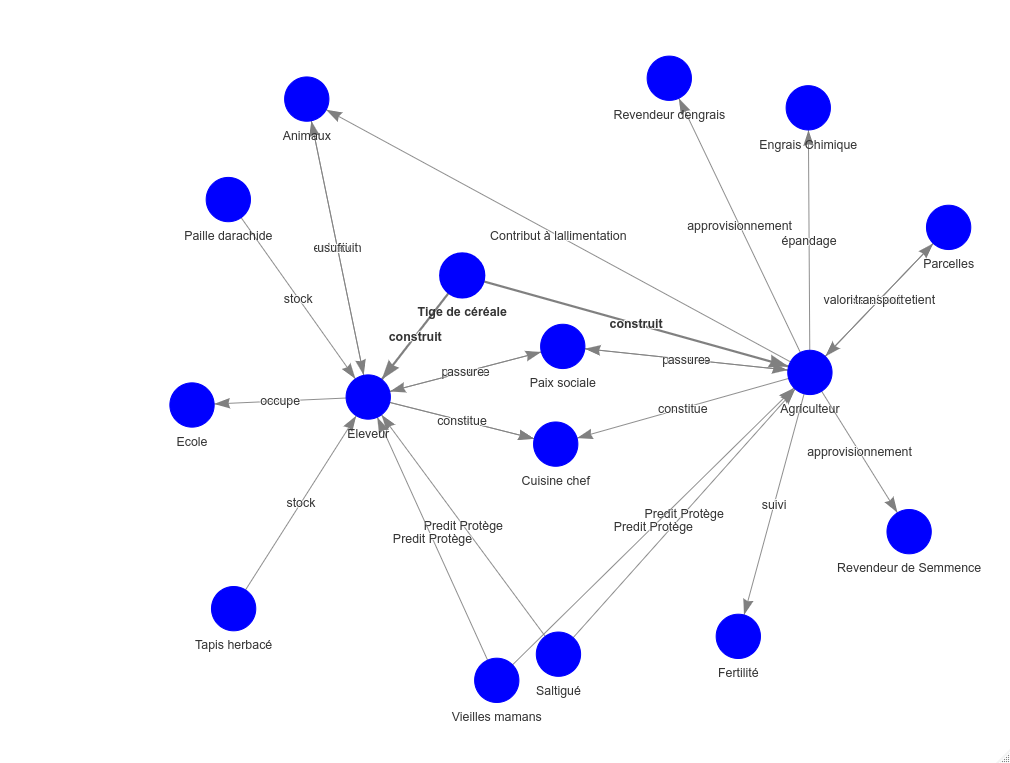
\includegraphics[width=0.9\textwidth]{img/agriculteur_eleveur.png}
  \end{center}
    %légende de l'image
  \caption{Sélections des relations entre agriculteur et éleveurs}
  \label{fig:agripasteur}
\end{figure}

\subsection{L'agriculteur}

\begin{paracol}{2}

  C'est lui qui s'occupe, prend soin et valorise la terre. Il a des interactions avec les revendeurs de semences et d'engrais chimique, même si ces derniers ne sont pas assez disponibles.

  La fertilité de la terre est un enjeu très important. Elle est suivie et perçue par les agriculteurs. L'exemple d'un quartier de Diohine qui s'est retiré temporairement de la jachère communautaire est éclairant à ce sujet :
  \begin{quote}
    Les habitants d'un quartier de Diohine voulaient pouvoir disposer de toutes leurs terres pour cultiver, y compris les parcelles normalement en jachère. Ils ont décidé de sortir de la jachère, ce qui peut s'expliquer par le fait qu'il n'y avait pas beaucoup d'éleveurs parmi eux, ils étaient donc moins sensibles aux enjeux de pâturage du bétail.

    Au bout de trois ans, ils ont réintégré la jachère du quartier et les processus collectifs d'orientation des cultures qui l'accompagnent. Ce qui veut dire qu'il sont rester 5 ans sans jachère (deux cycles). Les participants avancent deux types d'explication à ce revirement: d'une part la baisse des rendements constatés sur les parcelles sorties de la jachère, et d'autre part une dégradation de la paix sociale qui rendait la situation difficilement tenable pour le quartier qui s'était désengagé.
  \end{quote}

  L'agriculteur contribue à l'alimentation des animaux de l'éleveur en mettant à disposition les résidus de culture, que ce soit directement sur la parcelle ou sous forme de bottes de pailles de céréales récoltées.

\switchcolumn %Sérères

  Ten na topatwaa so a sutaa no lang ke o ndjirin, so a lokoor fo djidjikax ax kef o angare fe.

  O kaadel o len lang ke kaa ref kaa djieg na o ndjirin, ten taxu boo xoxoox we a saytuwan, we sutu ina na toss ake diohine a lalan in.

  \begin{quote}
    O Dik no saax le diohine a mbug a ndaaw lang den fop dax  da mbaag o ngoxaa den fop bo no xa kol axe ndef na na toss ake, kene tektaa ee dik faaga maye gaynaak, ten taxu boo ngaynaak nee soxal den.

    Nda no tig tadik nda numtuwid na toss ake kaaga tektu yee a mbi atig betik kaa da ndosser na, a nga a yee djiegel den kaa waniu u, to yiit djiam fe nda ndjieg ina fo sate fe it a waaniu.
  \end{quote}

O koxoox kaa fog no we na niowna mumen ke fo ke na yokaa no kol le, nen a kanga fake ta gada yaa ta saxad na baa djiut.

\end{paracol}

\subsection{L'éleveur / KAYNAAK OXE}

\begin{paracol}{2}
  L'éleveur est défini par les fonctions qui le lient aux animaux. Il les entretient et bénéficie de l'usufruit de l'élevage. L'éleveur est également lié aux pailles de céréale et au tapis herbacé par la fonction de stockage qui servira plus tard à nourrir les animaux.

  Par ailleurs un élément qui n'est pas visible sur le graphe est le lien qui existe entre le rôle d'agriculteur et celui d'éleveur. En effet dans la plupart des cas ces deux rôles sont occupés par la même personne. Mais quand l'agriculteur n'est pas éleveur, il confie des animaux à ce dernier qui a la charge de les entretenir et de les faire fructifier. L'éleveur est alors le banquier de l'agriculteur. On l'a abordé avec les questions des conflits; les agriculteurs gardent une part de responsabilité si leurs animaux font des dégâts sous le gardiennage de l'éleveur, ce qui accentue encore la relation de dépendance. Enfin on pourra souligner que tout le bétail d'un agriculteur n'est pas forcément confié au même éleveur. Ce qui permet d'accroître également les interdépendances.\\

  \switchcolumn %Sérères

  O kaynaak oxe a waa damtel fo ke fokatuna fo mumen ke, kaa topatoxaa den so a xotaa ten o ndjirin, a lokoora xina it fo dat le na kobale fo a kanga fake ta gada dax ta wag o niowitan yaa dad a niak na.

  Ten taxu a djiega ke ganuwerna nder lokoor ne djieg na nder o koxoox o xe fo o kaynaak oxe.

  Ke modji na o tax kene ka ke da mbiyaa den dik, o kiin o len kaa fi an, nda boo o koxoox a referna o kaynaak kaa yobo doxin o kaynaak mumenun so o xene a topatwaa den, yaag koy o kaynaak ten refu dap no koxoox, ten taxu o koxoox ne sutwaa no ndaawir ne yaa o kaynaak um a yakan na.

  \switchcolumn %Francais
  Le lien entre les agriculteurs et les éleveurs est un élément particulièrement important. Il repose et constitue le socle de la paix sociale. C'est un concept auquel les acteurs se réfèrent souvent.

  La paix sociale est un commun clef du système. Pour Aubert \textit{et al.} \cite{land_tenure_and_development_technical_committee_opportunities_2017}, un Commun clé est "celui [ou ceux] susceptible d’avoir un effet d’entraînement important sur la résilience des autres communs qui lui sont liés". Ici, les éleveurs et les agriculteurs ont des intérêts qui peuvent diverger. Si un déséquilibre survient, la communauté fera le nécessaire pour restaurer la paix sociale et assurer son maintien dans le temps. Les liens qui unissent les acteurs sont très forts, et d'autant plus forts qu'ils sont entretenus dans le temps et dans l'espace. La prise en charge des bergers, du bétail pour l'abreuvement ou de traitement des animaux malades matérialise ces liens de solidarité entre éleveur et agriculteur.

  \switchcolumn %Sérères

  So it I mbaa lay ee o koxoox a waa doxin gaynaak fogrer mumenum.
  Lokoor ke nder o koxoox fo o kaynaak kaa djieg na solo o, yam a waa ndetel ne na koor ndap djiam.
  Djiam kaa ref kaa fop a mbog na, to djiam fene kaa djieg dole no ken a fokataa fop, ganaak we fo xoxoox we ka ndjeg bug bug ke na xaadjia den, etn taxu boo a ndawra nga fop kaa mbexeyaa ndiofor den yam lokoor den ka magin bo ta xup, bo o andan o det ne o koxoox oxe dimle ta momol we na tal na le na yer na le bo no badin ne

\end{paracol}


\section{Structure de la résolution de conflit}

\begin{paracol}{2}
Nous avons voulu mettre un éclairage particulier sur la ou les structures de résolution de conflit. Ces conflits sont très majoritairement liés à la terre et aux fonctions et enjeux parfois contradictoires de l'élevage et de l'agriculture.

J.P. Jacob\cite{jacob_terres_2007} estime que les droits fonciers en Afrique sont à considérer comme une manière de rattacher les humains et non humains à l'existence. Ces droits fonciers traditionnels lient moins les surfaces que le droit à l'existence des actants en mettant la priorité à l'inclusion plutôt qu'à l'exclusion. Considérer le droit foncier comme moyen d'existence fait le lien avec "la zone critique" que définit Latour\cite{latour_face_2015}. Cette dynamique contribue donc à repousser la vision individualiste de la modernité qui place l'autonomie au centre de tout. Or, de manière curieuse, cette autonomie individuelle des modernes, ne tient pas du tout compte du réseau de solidarité entre humains et non humains qui la rend possible, et nie l'autonomie à laquelle une société peut prétendre collectivement.

Pourtant, et nous nous  attachons à le montrer dans la description des structures de résolution de conflit à Diohine, la prise en compte des réseaux de solidarité est omniprésente. Paul Séné nous dira même "ici nous dépendons tellement les uns des autres qu'on est bien moins libres que vous". Selon nous, la liberté dont parle Paul est en fait la recherche d'autonomie individuelle des modernes.


Nous avons extrait du diagramme général (fig. \ref{diagComplet}) la figure \ref{fig:conflict}

\switchcolumn %Sérères

Ka I mbugo bisiid o lerand na niadji not ale na kemband ale no tawir ke, yam ke modji na ten o may ka lokoor lang ke nder a kook fo ngaynaak.

J.P.Jacob\cite{jacob_terres_2007} a le, lang ken a afrik ka ref ke lokoor na wiin we, to a wa layel e ke modji na ten o djieg solo ten refu ke na roka ee ke na sutwaa, o dole na nga lang ke rek xan o bugo xass ke latour a lay na, bo a niadjinod ale ne ka sut o djiegwood o le, yam kene ka dole ne mbokatoor ne no wiin we.

Ko kene I mbagan o lalit na kemban ale no tawir ke diohine, ten taxu bo paul sene a lay ee in diohine o xu refna ko soxla o kend of.

Ten taxu no madarga ne I mbi na I sut ten, dik ta ref o kol fo ngel ne.
O kol le ref o djieg ole, ten taxu ndawir ne xan ta wadik kaa djioforan na o xe yakanena, a kenband a lene o xe ref ka it no waxtan.



\end{paracol}

\begin{figure}
  \begin{center}
    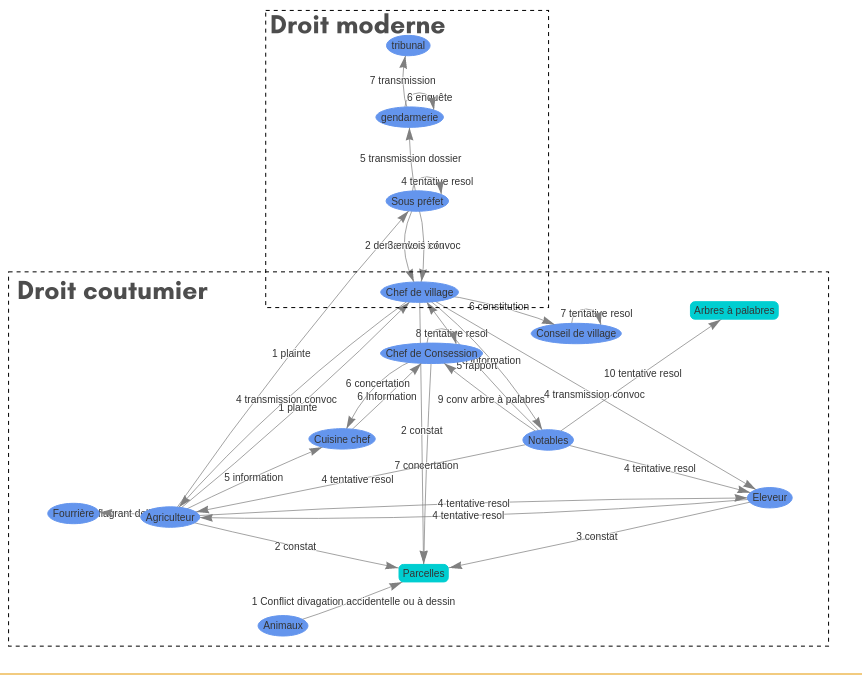
\includegraphics[width=0.99\textwidth]{img/zoneDroitConflits.png}
  \end{center}
  \caption{Selection des relations liées au conflit. Extraction du sous-graphe des arcs étiquetés "dynamique conflit" du fichier}
  \label{fig:conflict}
\end{figure}

\begin{paracol}{2}

  Deux ressources sont représentées sur ce sous-ensemble du modèle conceptuel : la parcelle, et l'arbre à palabre.

  La parcelle est le support du droit à l'existence (J.P. Jacob). Le conflit va donc chercher à résoudre un dommage causé par A (ou via A': les objets de A) au droit d'existence de B. Toutes les tentatives de résolution du conflit (4 sur le schéma) impliquent des discussions et des concertations à chaque étage de la structure sociale.

  Les animaux (A') de l'éleveur (A), ont causé des dommages sur la parcelle (B') de l'agriculteur B. L'agriculteur constate les dégâts, avec son chef de concession (au besoin). A et B vont tenter de résoudre le conflit sous l'autorité de leurs chefs de concession, si B refuse les compensations/amende honorables de A, le conflit est exposé au chef de village par l'intermédiaire du chef de concession. Le chef de village va pouvoir avoir recourt au Notable sous l'arbre à palabre de manière formelle ou informelle. À l'intégration de chaque nouvel acteur, B est sommé d'accepter la compensation de A pour rétablir la paix sociale. Si B se considère toujours lésé, il peut porter sa plainte auprès du sous-préfet. Celui-là peut demander l'avis rendu par le chef du village sur la base duquel il décide de transmettre le dossier à la gendarmerie qui établira une enquête avant de verser le dossier au tribunal.

  \switchcolumn %Sérères

  Mumen ke A o kaynaak A djiena a yakaa o kol B o koxook B djiegna, ten taxu bo A fa B def na yaal pind den xana mbexey a ngembador, nda o yaal mbind en B a fania nga xan yaal saax a djiem o lay fa B a fokat ten we ndjieg na xa niuxur no sax le no ngel na dax djiam a djieg, maga B xoxa nga a den xan te bind a plente a bisin ma superefe, so o xene xan ta laamit a yaal sate sa sur na kayta le sadarmori, den o da mbi lamit den sa surnin tirbinal.

  Latour ten tax ta lay ee a djiaga o kiin me o niowaa fo ken a niownorang ten tax ta lay kene a djiega diohine.

  Kene taxu ta lay ee xa pasong xa dak ndjiegu na kemband ale: me o niowa ref na ngentan ne, fo ken a niownorag ref na a dat

  \switchcolumn %Francais

  Latour (La zone critique, 2021), rappelle la distinction entre  un \textit{monde où l'on vit} et un \textit{monde dont on vit}. Le monde où l'on vit  est l'endroit où l'on inscrit ses gestes du quotidien, alors que le monde dont on vit est  celui dont on dépend pour vivre, celui dont sont tirées les ressources et les objets qui supportent ces gestes quotidiens.

  Cette distinction, entre \textit{monde où l'on vit} et \textit{monde dont on vit}, s'applique aux conflits de Diohine. Il y a deux échelles de résolution de conflit:  celle du monde où l'on vit qui s'étend jusqu'aux frontières du village et mobilise les acteurs locaux lors des tentatives de résolution de conflit à l'amiable accompagnées par les notables et le chef de village selon les lois du droit coutumier ; et celle du monde dont on vit, qui s'étend au-delà du village jusqu'aux instances d'autorité nationale et selon les lois du droit moderne positif.

  Pour H. Arendt\cite{arendt_condition_2020} l'Homme est plongé dans la \textit{vita activa} (en opposition avec la \textit{vita contemplativa}). La \textit{vita activa} est elle-même composée de trois éléments : le travail, l'\oe{}uvre et l'action. Le travail rassemble toutes les tâches qui sont essentielles à la survie des individus; les choses qui leur permettent de vivre et de perpétuer le cycle naturel (manger, se déplacer, \textit{etc.}). L'\oe{}uvre est "l'activité qui correspond à la non naturalité de l'existence humaine[...]. L'\oe{}uvre fournit un monde artificiel, nettement différent du tout milieu naturel." (p. 58). Enfin l'action "correspond à la condition humaine de la pluralité, au fait [...] qu'ils [des hommes] vivent sur terre et habitent le monde.[...] cette pluralité est spécifiquement \textit{la} condition [...] \textit{per quam} de toute vie politique."(p.60).

  \switchcolumn %Sérères

  ten taxu boo H. Arendt a lay ee o kiin ka rokaa no keta layaa vita active, sufalorna fo keta xoyaa vita contemplative, o perand oxe tadik fokatun: cialel, ke djialena, fo a pi ale.

  Cialel ke kaa fokat ke warena o niowit, ke djialena ka ref garanerna xoxum ta djieg, so a pi ale ka ref dole fe o kiin oxe atid na, ka nandit nen niowa tok lang so gen na adna.

  Yag koy bon gar na no tawir ke, we na mbi a ka ndef na pi ale ten tax ta wag o xembantel kam saax le, nda a suranga no wiin wa kaga refna cialel den we na mbi akam sate fe mbagka te ten tig.

  Bo ngel ne mbagerna ten tig xan ta surnel ma xup na ta ref na dat.

  Ten taxu serer a layaa ee xemban a telu, modjiu xemban na keen ta tekit ee xemban tin kam ngaak ne modjiu ta fad no ngel na.

  Bo ndawir ne a surna a yaal saaate ba fadid na superefe, ndawir naga ka sutu na saax ngemban taa so a ret no dat no maad, to anda yee a dat xupu doole ngel ne.

  Ten taxu bo ke modji na o may no lokoor ke a refa no we na mbi ra, ten taxu H. Arendt a lay ee o ndjirin polotik kaa lokoor it fo waxtaan fo djioktoor no kaa farna no ndawir, a lalta it lokoor ne refna nder o kiin fo wiin we.

  \switchcolumn %Francais
  Donc si on se place du point de vue du conflit, les acteurs locaux sont dans l'action au sens de H. Arendt, temps que le conflit est géré par la coutume. Quand il passe dans le droit conventionnel, le conflit se déplace dans la sphère du travail. Sa gestion est déléguée en dehors du \textit{monde où l'on vit} par des individus dont c'est le travail. Et les acteurs locaux sont eux dépossédés de l'action.

  Les acteurs organisés autour d’échelle de négociation locale et de l'arbre à palabre tentent par la concertation (\textit{Xartan} en Wolof) de résoudre le conflit. À chaque étape, `chef de concession`, `chef de village`, \textit{etc.} la victime est au centre de l'attention sociale. C'est à elle qu'il est demandé d'accepter l'amende honorable qui est faite par le contrevenant. Tant que ce n'est pas le cas, le contrevenant est exposé au niveau d'autorités supérieures.

  \begin{quote}
      "Il est préférable de régler un problème assis plutôt que debout" (proverbe sérère). \textit{il vaut mieux que le problème se règle discrètement dans la cuisine plutôt que sous l'arbre à palabre}
  \end{quote}


  Quand le conflit dépasse le chef de village pour arriver au sous-préfet, le conflit sort du domaine du droit traditionnel pour entrer dans celui du droit positif. Et le droit Postif domine le droit traditionnel. On passe donc dans le domaine du \textit{monde dont on vit}. Celui dont on dépend même à ses dépens.

  Le fait que la très grande majorité des interactions se tienne  entre des  acteurs (seulement deux ressources sont identifiées), met en relief l'importance du "politique" et du langage au sens de H. Arendt\cite{arendt_condition_2020}. En effet, par le langage au sein des différentes instances de discussion/négociation des conflits, le résultat de l'action va évoluer de l'intention originale. "Cette contrainte exprime la dépendance de l'activité individuelle à l'égard du réseau de relation humaine" (p.43, Paul Ricoeur, in H. Arendt\cite{arendt_condition_2020}).
\end{paracol}

\section{Structure et mécanique de gestion collective de l'espace / NE ANDONA E NEN A KOB ALE A SAYTOX TEL}

\begin{paracol}{2}
  Le territoire de la commune de Diohine se distingue des communes voisines par la survivance d'une gestion collective de l'espace. Une partie des terres de la commune est chaque année mise en commun en temps que la jachère collective. Cette jachère permet un repos de la terre et laisse des espaces à la veine pâture.

  Les animaux sont sous la surveillance d'un berger la journée et sont attachés "au piquet" la nuit pour profiter des amendements liés à la fumure. Les animaux sont gardés la nuit, et le berger s'abrite dans une petite hutte (c.f. fig. \ref{fig:photoJachere})

  Les espaces de jachère doivent être continus pour permettre aux animaux de se déplacer plus facilement et pour éviter les dégâts. Si une cuisine a un grand nombre de parcelles dans la jachère une année donnée, elle va se faire prêter ponctuellement des parcelles pour subvenir à ses besoins par les autres membres de la communauté.

  La zone de jachère n'est pas une zone d'exclusion de la culture. On y inverse simplement la charge de la surveillance du bétail. Dans les zones cultivées, c'est au berger de faire attention à ce que le bétail ne rentre pas dans les parcelles. Si d'aventure une parcelle était mise en culture dans la jachère communautaire, la charge de la surveillance serait au cultivateur.

  L'évolution de la démographie et des pratiques culturelles et culturales fait qu'aujourd'hui la jachère est régulièrement "rognée". Cette diminution des surfaces se fait par les bords qui sont moins exposés qu'une parcelle cultivée seule et entourée de jachère.

  Pour les acteurs, la survivance de la jachère est en partie liée à l'histoire du peuplement de Diohine. Initialement constituer de peu de famille, les arrangements sont plus faciles. Ces familles étaient assez homogènes en termes de pratique : tous agro-pasteurs. Il y a donc une conscience forte de l'importance du bétail pour restituer la fertilité aux champs.

  La saison des cultures et l'organisation du territoire qui en découle, sont lancées au moment de la première chasse. Seront définis à ce moment-là les espaces de culture, et c'est à partir de ce moment là que les prêts de parcelles pourront avoir lieu.

  Extraction du sous-graphe des arcs étiquetés  "interaction" du fichier DOT \url{https://github.com/ElCep/DSCATT/blob/master/PARDi/diagram_pardi_simple_edges.dot}

\switchcolumn %Sérères

  A saytax ale na kob ale diohine kaa gutair fo ne andona ee sate lakas ke a mbi ta, a kadji na kob ale ka xadjiel a toss, a toss a lene ka niot na lang ke so a niowna mumen ke, gaynaak we ka ngay ta natoss ake so yeng anga da mbe no xa sir den.

  A toss ake kaa mbar ciodadir dax mumen ke a mbago mbirlu waa to yakanke o leng, nda boo ngaak a dieg na xa kol xa mayu na toss ale, kaa xedikaa yaal kaak lakass ma ta xoox na, a toss refe yee ta fanit o xooxel soom nda ka niowna mumen ke itam, nda yit o kaynaak oxe ka war o deta den boo yakan ke o kiin, nda yit bo o koxoox a xoox na kan a toss ake ten waru o gaynaakaa o kolum.

  Wiin we may na a taxa boo a toss ake a mbaniuwaa na xa saax axe, we i mbaxtaanta ka lay ee wiin mayu we taxu a toss ake a ngaynaakel, nda koy ne mbasil ke fop a mbog na a taxa boo tawir ken aa yobaa o ngembadel yam den fop xoxoox fo gaynaak a ndef to a anda yo ndjirin mumen no lang, baa miis nay o mene a layta yo me a toss ake a def kaa, so we mbarna ngedik xa kol a ngedik.

\end{paracol}


\begin{figure}
  \begin{center}
    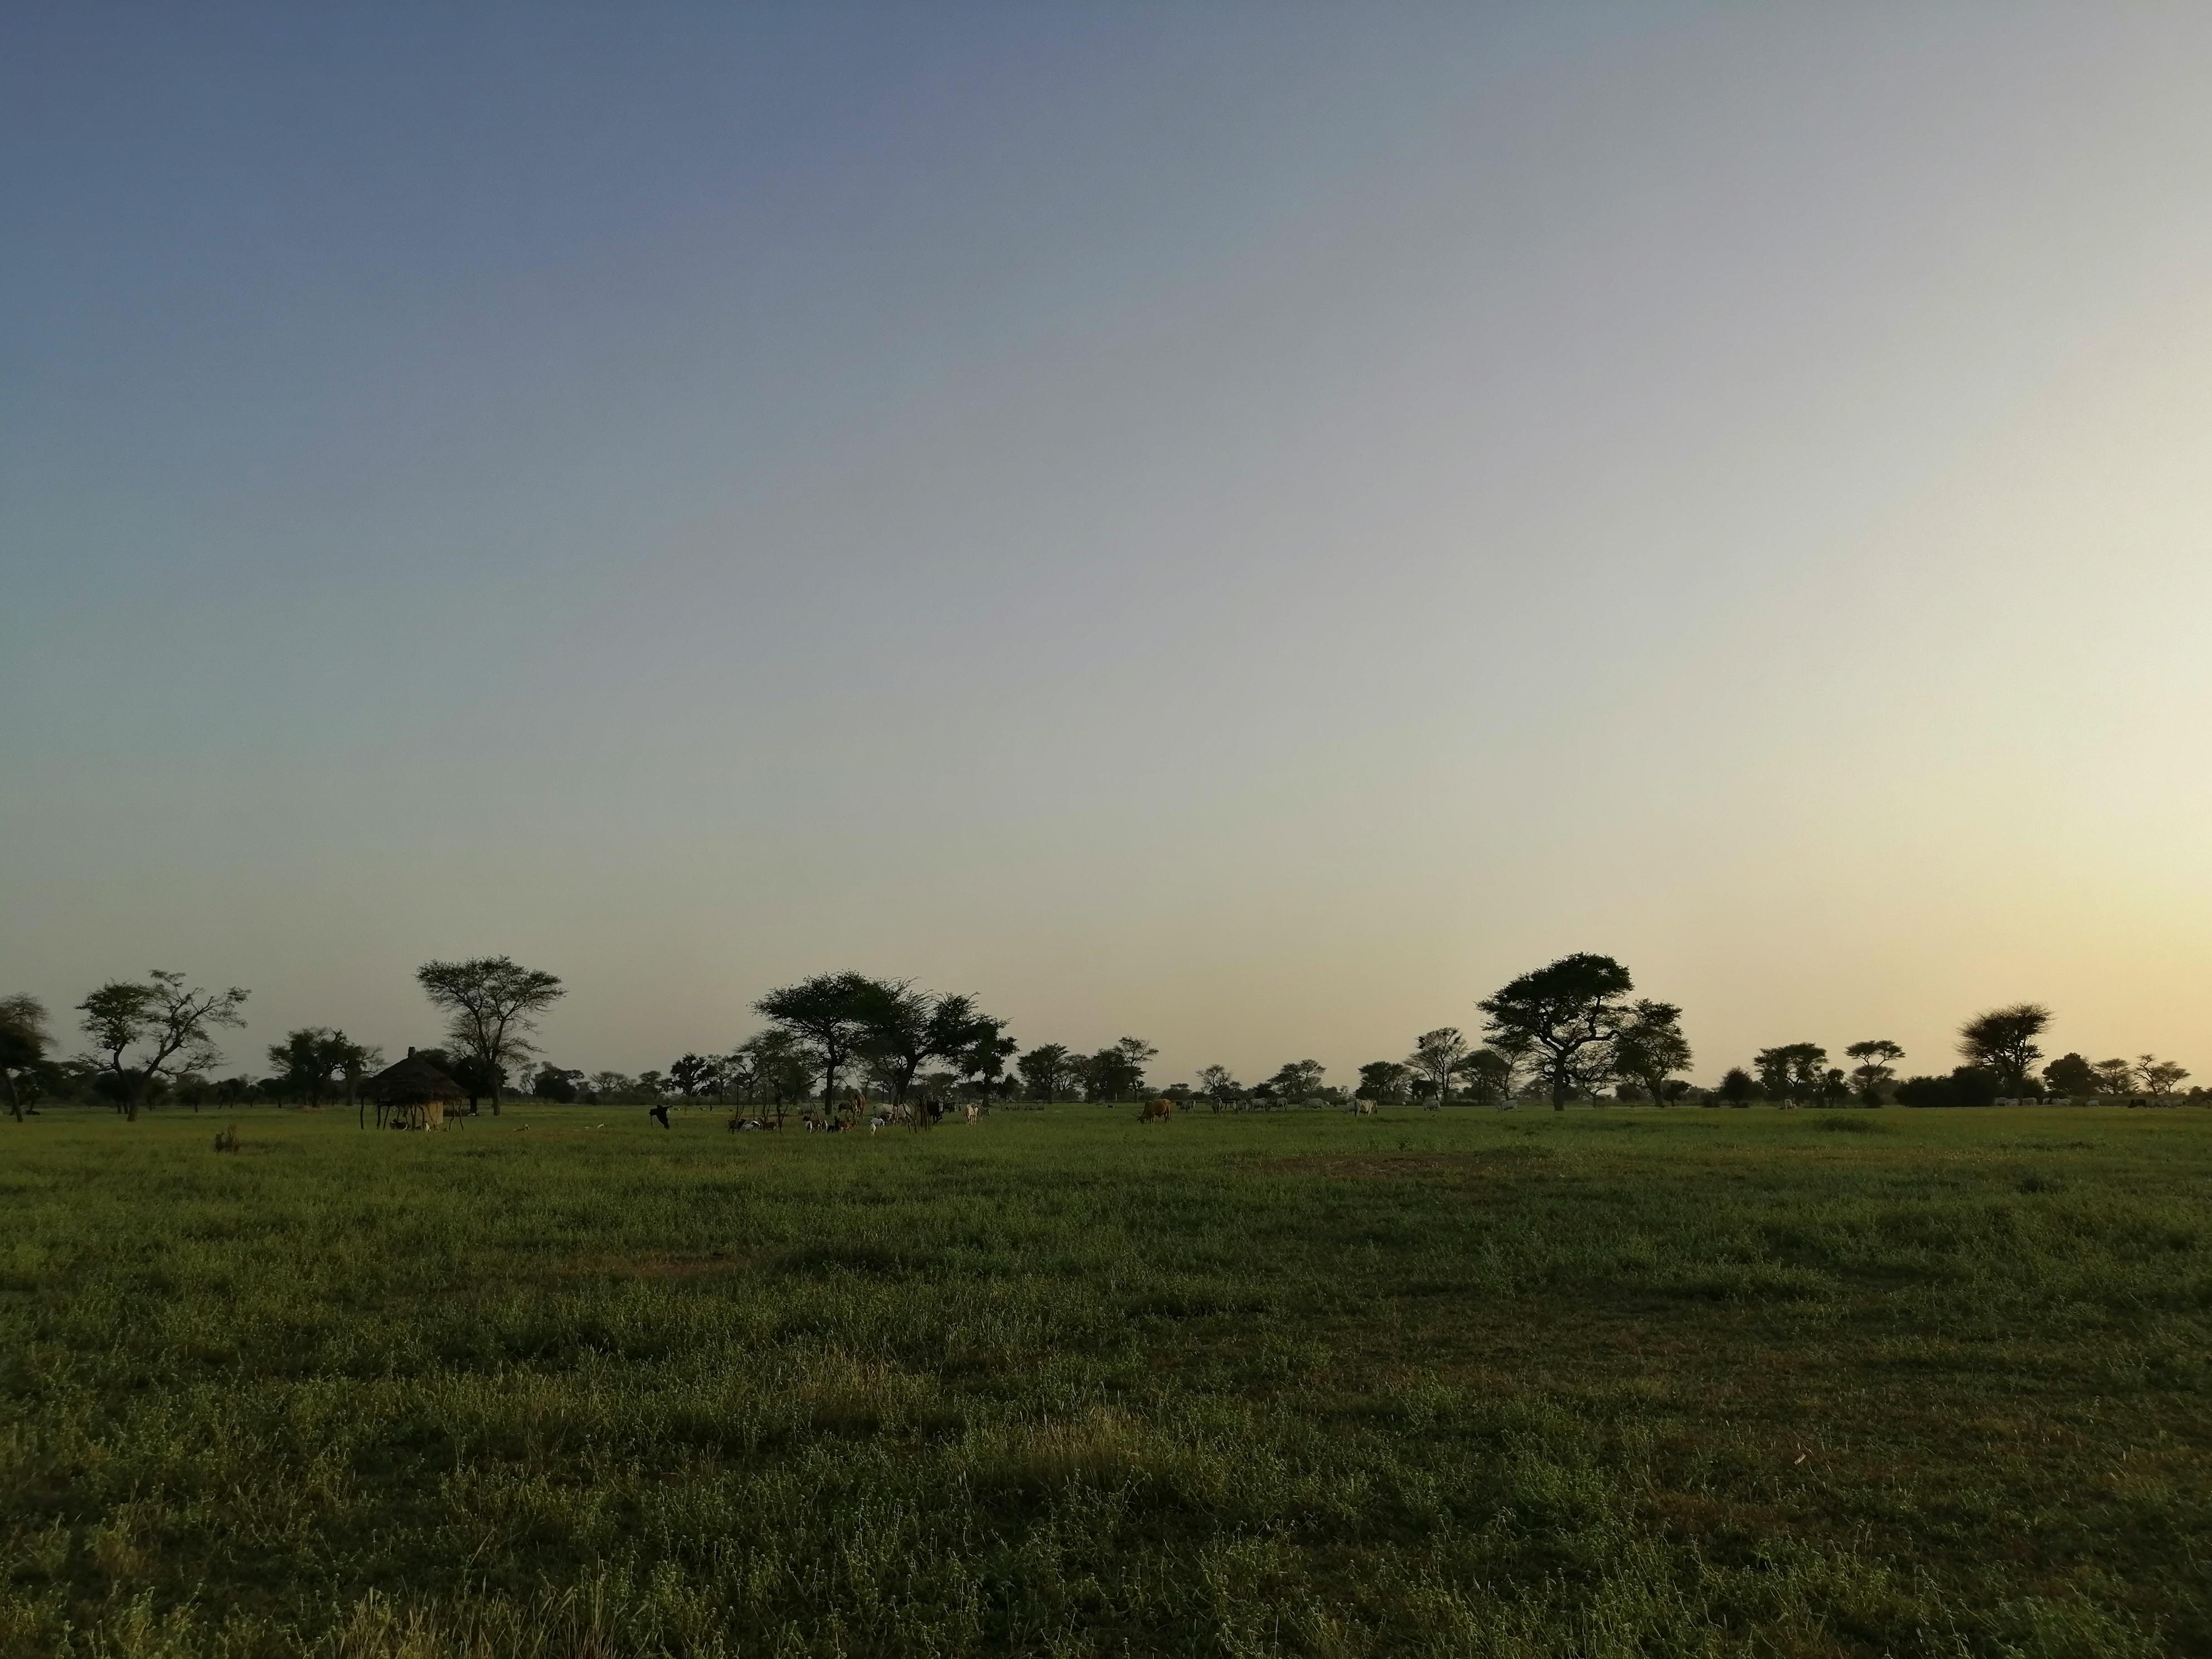
\includegraphics[width=0.9\textwidth]{img/jachere.jpg}
  \end{center}
    %légende de l'image
  \caption{Jachère au Nord de Diohine (photo prise en octorbe 2021)}
  \label{fig:photoJachere}
\end{figure}



 \subsection{Mise en commun : la première chasse / A TAM ALE NO MIIS OLE}\label{sec:premierchasse}

 \titlebox{\textit{Les saltigués}}{
   La cérémonie divinatoire du xooy est organisée à l’approche de la saison des pluies sur la place des villages par la communauté des Serer du centre-ouest du Sénégal. Durant cette longue veillée nocturne, les maîtres voyants, connus sous le nom de saltigués, se succèdent dans le cercle qui leur est réservé pour délivrer, au rythme des tamtams, leurs prédictions à une assistance en délire. La cérémonie du xooy apporte des réponses aux questions clés pour la communauté que sont, entre autres, la pluie, les fléaux ou les maladies et les remèdes.\footnote{Source : \href{https://ich.unesco.org/fr/RL/le-xooy-une-crmonie-divinatoire-chez-les-serer-du-sngal-00878}{site de l'unesco}.}
 }

 \begin{paracol}{2}
   Cet événement annuel est constitué de trois temps forts :
   \begin{enumerate}
     \item La réunion nocturne, qui regroupe les hommes : les voyants "\textit{saltigués}" et ceux «qui ont des dons », partagent leur prédiction, et leur connaissance sur l'année à venir, les grandes tendances, si des calamités sont à prévoir. Ils identifient les solutions et les libations à faire. Ce sont ces informations qui seront centralisées par le grand saltigué.
     \item Première chasse. Elle concerne plusieurs villages.  Le grand \textit{saltigué} centralise les informations, des autres \textit{saltigués} et fait un message à tout le monde, avec des recommandations. Les hommes partent à la chasse dans la brousse, les anciens restent à discuter sous l'arbre à palabre. C'est un moment important de la transmission de connaissances, chaque quartier dispose d'un délégué qui rapporte au saltigué les informations sur sa zone, son quartier.
     \item La réunion diurne le même jour que la chasse a pour objet de définir les orientations des cultures et négociations d'accès à la terre. Il y a une réunion par quartier de Diohine et les informations sont ensuite centralisées, et les zones de jachère, d'arachides et de mil sont définies.
   \end{enumerate}

   \switchcolumn %Sérères
   Bo ndig a matid na ka ndjiegaa o xoy, so saltiki ke kaa ndokaa so a lay no kaa farna no fof le no yak fo kaa waag na o xemban. O xet o lene a waa xadjiel a kaadji a tadak

   \begin{enumerate}
     \item waxtaan le no goor we o yeng ole so saltiki ke a lay ke da nga na, ku warna o saafaara el sadax a fiel, so ta layel a saltiki fa maak fee.
     \item o miis ole sate mayu mbogun so maga saltiki fa maak fe a layit ka ke ga e na, so goor we a ndet a miisik, maak we moof a ciunga da gatid, maaga saltiki yoo saltiki a layaa ke ta ga na
     \item no waxtaan le no niaal ne mene a toss ake a degit kel, tufedufe ke layel me da ndef kaa fo ked ale no xa kol axe, diko dik kaa mbaxtaanaa kam dem.
   \end{enumerate}

   Ten taxu o miis o lene kaa war o madel, yam mumen ne refna o xoss ole teen a andel.
O Miss ole fafanga nda mbigok so a tup ale damel, nieniebaan ne djiawel da mbetu.

 \end{paracol}

\subsection{Interaction dyadique : le prêt de terre / A LUB ALE NO XA KOL AXE}

\begin{paracol}{2}
  Une fois que le zonage est effectué lors de la réunion diurne, les tractations pour obtenir des parcelles peuvent commencer. Ce sont des négociations qui se font dans la discrétion des cuisines et sont très largement tributaires du réseau de solidarité que les uns et les autres sont capables de mobiliser (c.f. infra).

  Les parcelles sont prêtées par le chef de cuisine pour une durée d'un an. Les prêts étaient traditionnellement accompagnés d'offrande/cadeau en nature. Mais de plus en plus ces pratiques se métamorphosent en location (prêt contre de l'argent).

  \switchcolumn %Sérères

  Bo a toss ake degena boo a djut, a lub ale no xa kol axe comaase, a lub alene, o xe fitel nder kaak kef o no sutura, yaal kaak ke nab anta xa kol, nda no xiid soom a refa, o band ange o kol koo djiokoogu o yaalum a djial o ciodin no ke xoxoona, nda diiki koy ke modji na o may xaalis na ciodtatel

\end{paracol}


\section{Les réseaux de solidarité}

% \titlebox{\textit{warning}}{
%   Est-ce que la solidarité ici est proche/assimilable à la notion de proximité de l'école des proximités (Tores, Grossetti, Bouba-olga)
%
%   [paul]Pour Grosseti que je situe vaguement, je pense qu'on peut parler d'encastrement, je ne connais pas l'école des proximités.
%
%   [paul] Les interactions listées précédemment s'inscrivent dans différents réseaux de solidarité, solidarité étant ici entendue au sens de la relation qui peut exister entre des acteurs partageant le même contexte d'action collective, et reconnaissant l'obligation d'assistance qui lie les membres du groupe auquel ils appartiennent.
%
% }

\begin{paracol}{2}
  Différents réseaux de solidarité existent de manière imbriquée et enchâssée les uns dans les autres. Nous proposons de distinguer trois types de solidarités selon la nature des ressources qui fondent les interactions et leur portée.

  On pourra d'abord distinguer des solidarités spatiales, de courte portée,  mobilisées lors des négociations et des discussions annuelles récurrentes ( prêt de terres en cas d'insuffisance, orientation des cultures, aménagement des couloirs pour le passage du bétail) ou ponctuelles (garde de troupeau, prêt d'animal de trait, d'outil).
  Ce réseau est un réseau qu'on pourrait qualifier de réseau de voisinage, puisqu'il comprend les cuisines d'un même groupement de quartiers.

  Le second réseau qui se sur-impose au réseau de voisinage, mobilise des acteurs plus éloignés : des membres des cuisines d'autres groupements de quartier.
  Les interactions sont plus ponctuelles : conseils sur l'achat ou la vente de bétail, prêts d'argent, soin au bétail, renouvellement d'outils. Exemple : mobilisation générale du village pour cultiver et récolter en cas de maladie d'un paysan.
  Enfin un troisième réseau de solidarité, plus étendu, est celui qui lie les cuisines à leur famille lointaine, installée dans les villes de taille plus importante, voire d'autres pays (diaspora).
  Ce réseau est le support d'interactions  moins fréquentes, et il semblerait qu'il soit mobilisé principalement pour contribuer financièrement à la sécurité alimentaire des familles du village, ou à statuer sur des évènements politiques majeurs. (La diaspora mondiale peut même être convoquée pour certains évènements majeurs de la vie du village)

  \begin{quote}
    "Il y a de la solidarité en face de l’insuffisance. En cas de maladie d’un paysan, le village se mobilise pour cultiver et récolter. De la nourriture est glissée sous la porte, les greniers sont remplis de nuit, sans le dire. La discrétion est importante ! "
  \end{quote}

  \switchcolumn %Sérères

  Ndamtir maak a djiega nder wiin we, boo a waa xaaadjiel a ciaf a tadak: Ndamtir ne na lub ale no lang ke boo wiin we a deg na a toss ake, fo ne tufedufe ke a ndufitkel, a degale no xa cioc xa kayel axe, a lub ale no ciegel kooxir kef o no masin ke, a lub alene a waa layel eek am ngentan ne a dieg ta.

  A lub a dikander ale modjiu yaadji, yam ten modjiu god, yam a ref nder saate fa saate no kaa farna na ciik ciegel, a lub xaaliis, a sof masin koxiir, boo na sim ake da mbi a ndax da ndimle oxaa djir na.

  Ndadkander ne ref lokoor ne djieg na nder den fo o fog ole refna no teeru ke mbat bitimrew,wene a na ndimle ta yaa da ciodtaa xaalis dax da ndjik o niow, mbaat no kew ken a ndjiegaa.

  Mdamtir it a djiega yaa o kiin a djir na, saate fa ngar a ngooxanong a saxadanog, mbat o cioodel o niow na sutura too o leng yegkiran.


\end{paracol}
